%%%%%%%%%%%%%%%%%%%%%%%%%%%%%%%%%%%%%%%%%%%
%THIS FILE CONTAINS ALL COMMON COMMANDS NEEDED FOR COMPILATION INTO BOTH PDF AND HTML.
%THE EXTENSION file src/macros.sty CONTAINS ONLY COMMANDS NEEDED EXCLUSIVELY FOR COMPILATION INTO PDF
%THE DIRECTORY src/hva/ CONTAINS ONLY COMMANDS NEEDED EXCLUSIVELY FOR COMPILATION INTO HTML WITH HEVEA, WITH THREE EXTENSION FILES, imakeidx.hva, macros.hva AND picins.hva.
%%%%%%%%%%%%%%%%%%%%%%%%%%%%%%%%%%%%%%%%%%%
% 2024/04:
% - \documentclass[] : change {book} to {scrbook} from KOMA-script -> rewritting the manual.
% - change fancyhdr to scrlayer-fancyhdr (compatibility with scrbook) to scrlayer-scrpage (contained in koma-script) -> modify macros.sty too.
% - rewriting title page for \maketitle (use with pandoc [produce html file], \begin(title)...\end(title) doesn't work with pandoc, "microtype" package too)
% 2024/10
% - renaming chapter files with an order number
% - clean documentclass / packages / add comments
% 2024/10
% - comment \ifIllustration to always have pictures in manuel
% - texlive-extra-utils -> make4ht
% 2024/11
% - simplification of \usepackage{graphicx} when pdf

%\ifx\pdfoutput\undefined		% if no pdfLaTeX outputting
% test KOMA-script with "scrbook" instead of "book"
%\documentclass[%
%	paper=a4,			% default=a4 and therefore not needed
%	12pt,				% default=11pt
%	headsepline,		% line under the header
%	footsepline,		% line above the footer
%	twoside=semi		% same left/right margins, default=twoside
%]{scrbook} 			% 
%}{
%\else							% else pdfLaTeX outputting
\documentclass[%
pdflatex,
a4paper,			% default=a4 and therefore not needed
12pt,				% default=11pt
ngerman,			% use in babel, translator and varioref packages options %TODO: change with ngerman/english option in de/en manuals
toc=listof,			% add a "lof" (list of figures) line at the begining of the toc (table of contents)
twoside=semi,		% same recto/verso margins similar to simple verso margins, default=twoside
headsepline,		% draw rule below header
footsepline,		% draw rule above footer
plainfootsepline 	% draw footsepline on plain pages (here for heading pages, may be due to twoside=semi in scrbook options
]{scrbook} 				% KOMA-Script class "book"		
%}
%\fi

%\usepackage{ifpdf}					% detect pdfTeX, replaced by \Ifpdfoutput (KOMA-script)
\usepackage[T1]{fontenc}			% the font encoding
%\usepackage[utf8]{inputenc}			% no longer need to specify, included in LaTex since April 2018
\usepackage{lmodern}				% Latin Modern police
\usepackage{babel}					% use the language define in \documentclass
%\def\frenchcontentsname{Sommaire}	% rename "Table des matières" (at end of document) from [french]{babel} to "Sommaire" (at start of document)
%\frenchsetup{ItemLabeli=\textbullet}	% change 1st level list marker of french babel
%\frenchsetup{ItemLabelii=-}			% change 2nd level list marker of french babel
\usepackage{translator}		% for translating the Fixed Names
\usepackage{textcomp}				% for special characters like \textcurrency
%\usepackage{txfonts}
%\usepackage{ae}
%\usepackage{cmbright}
%\usepackage{times}					% changed from txfonts
\usepackage{newtxtext}				% install texlive-fonts-extra, replacing times which replaces txfonts
%\usepackage{lwarp}					% produce html file with lwarp (install texlive-extra-utils)

\usepackage{microtype}				% Font expansion (use for title) with "\textls[x]" - doesn't work with pandoc / espace entre caractères (utilisé pour le titre)
% Web addresses
%\usepackage{url}					% loaded by hyperref



% --------------------------------------------
% Load graphicx package with pdf if needed
% --------------------------------------------
%\ifpdf
%%\Ifpdfoutput{%
	%%\usepackage[pdftex]{graphicx}		% enhanced support for importing graphics (x=enhanced) and then using the \includegraphics command to insert the file
	%%}{%			
	% else								% Commented out to avoid errors in html, and put in the macros.sty file for pdf
	\usepackage{graphicx}				% enhanced support for importing graphics (x=enhanced) and then using the \includegraphics command to insert the file
	\newcommand{\refimage}[1]{ (fig. \vref{#1})}	% for the hypertext link display on images
	\newcommand{\vspacepdf}[1]{\vspace{#1}}			% for spaces after images bordered with text
	%%}
%% Graphics Extensions
%\ifpdf
%%\Ifpdfoutput{%
	%%\DeclareGraphicsExtensions{.pdf,.png,.jpg}
	%%}{%
	%\else
	%%\DeclareGraphicsExtensions{.eps}
	%%}
%\fi

% For illustrations
%\usepackage{picins}				% for text around image TODO change to wrapfig2 in the manuel
\usepackage{wrapfig2}				% TODO change in chapters, for text around image (replace picins)
\usepackage{caption}				% for good references in table of figures


%\usepackage{scrlayer-fancyhdr}		% facilities for constructing headers and footers, replace fancyhdr
% change to scrlayer-scrpage here and in macros.sty


%\pagestyle{fancyplain}
%\usepackage{tabularx}
%\usepackage{hhline}				% produce single or double line
%\usepackage{layout}				% TODO: Only if DE mode
\usepackage{varioref}				% defines the commands \vref, \vpageref, \vrefrange, and \vpagerefrange in french
%\usepackage{lastpage}
%\usepackage{longtable}
\usepackage{color}					% for a colored title page
%\usepackage{vmargin}				% for changing the title page margins
\usepackage{thumbpdf}				% create thumbnails (vignettes) in pdf


%\usepackage{emptypage}		% change by using \cleardoubleemptypage (in koma-scripts)
% Latex loads macros-3.0.sty for pdf output and Hevea loads /hva/macros.hva for html output
%\usepackage{macros-3.0}

%% Page layout %%
\usepackage[%
%	showframe,					% to see frame of geometry package
top=1in,					% marge haute
headheight=7mm,				% hauteur en-tête
headsep=6mm,				% distance entre entête et corps de texte
textheight=252mm,			% textheight=paperheight-topmargin-headheight-headsep-footskip
footskip=11mm,				% distance entre bas de pied de page et bas du corps de texte
hmargin=25mm				% horizontal margins (left and right), textwidth = paperwidt - margins
]{geometry}
\usepackage{scrlayer-scrpage}	% define and manage page styles by controlling page headers and footers			
\clearpairofpagestyles			% remove the default marks of the headings and the plain pages
\lehead{\leftmark}				% leftmark at left of even page
\lohead{\leftmark}				% leftmark at left of odd page
\rehead{\rightmark}				% rightmark at right of even page
\rohead{\rightmark}				% rightmark at right of odd page
\cfoot*{\pagemark}				% pagemark in the center of the footer
\ModifyLayer[addvoffset=-1ex]{scrheadings.foot.above.line}		% shift line up to increase distance between footer text and footerline in normal stylepages
\ModifyLayer[addvoffset=-1ex]{plain.scrheadings.foot.above.line}	% shift line up to increase distance between footer text and footerline in plain style page (chapter page)

%% Footnotes %%
\usepackage[%
perpage						% resets footnote numbering for each page of the document.
]{footmisc}						% provides several different customizations of footnotes

\renewcommand\footnoterule{%	% redefine rule above footnote
	\kern 5pt 					% above footnoterule, space between text and footnoterule  
	\hrule width 2.5in			% define rule's width to 2.5 in
	\kern 6pt					% space between footrule and footnotes below
}

%% Index %%
\usepackage[%
xindy						% sort index
]{imakeidx}						% for creating an index
\usepackage[%
columns=2,					% default value is 2
rule=1pt,					% thickness of a vertical rule between index columns. Default value is 0 pt, i. e. no rule.
totoc						% add index in toc
]{idxlayout}					% key-value interface to configure index layout parameters

\usepackage[unicode]{hyperref}		% replace \usepackage{url}, used to add an URL and rewrite the "grisbi-manuel-urldef.tex" file (must be the last package)
\hypersetup{%							% to create metadata to insert in pdf
	pdftitle={Manuel de Grisbi},		% sets the document information Title field
	pdfauthor={The Grisbi Team},		% sets the document information Author field
	pdfcreator={Alain PORTAL}			% sets the document information Creator field
	pdfpagemode=UseOutlines,			% set default mode of PDF display, UseOutlines=show bookmarks
	pdfstartview=XYZ null null 1.0,		% set the startup page view, XYZ=left top zoom
	pdffitwindow=true,					% resize document window to fit document size, default=false
	pdfcenterwindow=true,				% position the document window in the center of the screen, default=false
	bookmarksnumbered=true,				% put section numbers in bookmarks, default=false
	bookmarksopen=true,					% open up bookmark tree, default=false
	colorlinks=true,					% color links, default=false
	citebordercolor=1 1 1,				% the color of the box around citations, rgb color
	linkbordercolor=1 1 1,				% the color of the box around normal links, rgb color
	linkcolor=blue,						% color for normal internal links, color=blue
	menubordercolor=1 1 1,				% color of border around menu links, rgb color
	urlbordercolor=1 1 1,				% color of border around URL links, rgb color
	urlcolor=blue,						% color of URL links, color=blue
	plainpages=true					% do page number anchors as plain Arabic, default=false
	%	pdfpagelabels=true					% set PDF page labels - Commenté car élimine  "Package hyperref Warning: Option `pdfpagelabels' has already been used,"
}
%%%%%%%%%%%%%%%%%%%%%%%%%%%%%%%%%%%%%%%%%%%%%%%%%%%%%%%%%%%%%%%
% Contents: The url chapter
% $Id: grisbi-manuel-urldef.tex, modified from previous file :
% $Id: grisbi-manuel-urldef.tex, v 0.8.8 2011/XX/XX Jean-Luc Duflot
% $Id: grisbi-manuel-urldef.tex, v 1.0 2014/02/12 Jean-Luc Duflot
% $Id: grisbi-manuel-urldef.tex, v 3.0 2024/04/07 Dominique Brochard: create
% $Id: grisbi-manuel-urldef.tex, v 3.0 2024/11 Dominique Brochard:
% - rename file to 31-xxx
% - modify \urldef{\urlListSF} to {\urlListDiffGrisbi}
% - update Martin Stromberger mail
%%%%%%%%%%%%%%%%%%%%%%%%%%%%%%%%%%%%%%%%%%%%%%%%%%%%%%%%%%%%%%%


\urldef{\urlGrisbi}%
\url{https://en.grisbi.org}

\urldef{\urlGrisbiTelechargement}%
\url{https://en.grisbi.org/post/Download}

\urldef{\urlBugTracker}%
\url{https://www.grisbi.org/bugsreports/}

\urldef{\urlGrisbiWiki}%
\url{https://github.com/grisbi/grisbi/wiki}

\urldef{\urlTuxFamily}%         % French website
\url{https://www.tuxfamily.org/en/main}

\urldef{\urlSourceForge}%
\url{https://sourceforge.net/projects/grisbi/files/}

\urldef{\urlSourceForgeDocumentation}%
\url{https://sourceforge.net/projects/grisbi/files/Documentation/}

\urldef{\urlGitHubGrisbi}%
\url{https://github.com/grisbi/grisbi/}

\urldef{\urlLinuxGraphic}%         % French website
\url{https://www.linuxgraphic.org}

\urldef{\urlFramasoftLogiciels}%         % French website
\url{https://framalibre.org/}

\urldef{\urlFreeSoftwareDirectory}%
\url{https://directory.fsf.org/wiki/Main_Page}

%\urldef{\urlAssociationsGouv}%
%\url{https://www.associations.gouv.fr/la-comptabilite-associative.html}

%\urldef{\urlPlanComptable}%
%\url{https://www.plancomptable.com/index.htm}

%\urldef{\urlPlanDeComptes}%
%\url{https://www.plancomptable.com/titre-IV/titre-IV_chapitre-III_section-1.htm#431-1}

%\urldef{\urlListeComptes}%
%\url{https://www.plancomptable.com/titre-IV/liste_des_comptes_sa.htm}

%\urldef{\urlMaisonAssociations}%
%\url{https://www.loi1901.com/regle_comptable.php}

%\urldef{\urlComptaOnLine}%
%\url{https://www.compta-online.com/plan-comptable-general-pdf-ao2428}

\urldef{\urlWikipedia}%
\url{https://en.wikipedia.org/}

\urldef{\urlMetonymyDef}%
\url{https://literarydevices.net/metonymy/}

%\urldef{\urlAndrePascualEmail}%
%\url{andre@linuxgraphic.org}% without the leading "mailto:" for the DVI version

%\urldef{\urlDanielCartronEmail}%
%\url{daniel@cartron.org}    % without the leading "mailto:" for the DVI version

%\urldef{\urlCedricAugerEmail}%
%\url{cedric@grisbi.org}     % without the leading "mailto:" for the DVI version

%\urldef{\urlSebastienBlondeelEmail}%
%\url{sbi@april.org}% without the leading "mailto:" for the DVI version

%\urldef{\urlGeraldNielEmail}%
%\url{gerald@grisbi.org}% without the leading "mailto:" for the DVI version

\urldef{\urlBenjaminDrieuEmail}%
\url{benjamin@drieu.org}     % without the leading "mailto:" for the DVI version

%\urldef{\urlDionysosEmail}%
%\url{dionysos@grisbi.org}     % without the leading "mailto:" for the DVI version

%\urldef{\urlJulietteEmail}%
%\url{juliette@grisbi.org}     % without the leading "mailto:" for the DVI version

\urldef{\urlFrancoisTerrotEmail}%
\url{grisbi@terrot.net}     % without the leading "mailto:" for the DVI version

%\urldef{\urlLoicBreillouxEmail}%
%\url{lbreilloux@users.sourceforge.net}    % without the leading "mailto:" for the DVI version

\urldef{\urlPierreBiavaEmail}%
\url{pierre.biava@orange.fr}     % without the leading "mailto:" for the DVI version

\urldef{\urlDidierChevalierEmail}%
\url{didier.chevalier35@gmail.com}     % without the leading "mailto:" for the DVI version

\urldef{\urlWilliamOllivierEmail}%
\url{guneeyoufix@gmail.com}     % without the leading "mailto:" for the DVI version

%\urldef{\urlMickaelRemarsEmail}%
%\url{grisbi@remars.com}     % without the leading "mailto:" for the DVI version

\urldef{\urlJeanLucDuflotEmail}%
\url{jielbil@mailo.com}     % without the leading "mailto:" for the DVI version

\urldef{\urlAlainLetientEmail}%
\url{al1.letient@free.fr}     % without the leading "mailto:" for the DVI version

%\urldef{\urlGuyLebegueEmail}%
%\url{guy@guy-lebegue.fr}     % without the leading "mailto:" for the DVI version

\urldef{\urlMicheleBondilEmail}%
\url{ciboulette05@club-internet.fr}     % without the leading "mailto:" for the DVI version

\urldef{\urlListInfoEmail}%
\url{info@listes.grisbi.org}     % without the leading "mailto:" for the DVI version

\urldef{\urlListDevelEmail}%
\url{devel@listes.grisbi.org}     % without the leading "mailto:" for the DVI version

\urldef{\urlLudovicRousseauEmail}%
\url{ludovic.rousseau@gmail.com}     % without the leading "mailto:" for the DVI version

\urldef{\urlDominiqueBrochardEmail}%
\url{dbro17@free.fr}     % without the leading "mailto:" for the DVI version

\urldef{\urlBobAndersonEmail}%
\url{www23@scilutions.co.uk}     % without the leading "mailto:" for the DVI version

\urldef{\urlMartinStrombergerEmail}%
\url{mstromberger@mailbox.org}     % without the leading "mailto:" for the DVI version

\urldef{\urlListTraductionEmail}%
\url{traduction@grisbi.org}  % without the leading "mailto:" for the DVI version

\urldef{\urlListBugsreport}%
\url{bugsreports@listes.grisbi.org}     % without the leading "mailto:" for the DVI version

\urldef{\urlListDiffGrisbi}%
\url{https://listes.grisbi.org/mailman/listinfo}     % without the leading "mailto:" for the DVI version


		% include the "grisbi-manuel-urldef" file during the compilation

%% Glossary %%
\usepackage[%
xindy,              % sort glossaries
toc                 % add the glossary reference to the toc (table of contents)
]{glossaries}       % create a glossary, must be loaded AFTER hyperref
\usepackage[%
automake
]{glossaries-extra} 	% check why no glossaries and give solutions

%% Index %%
\makeindex  %[intoc]	% creates the index with its reference in the toc

\definecolor{jaunegrisbi}{rgb}{1,1,.6}			% creating your own colors {yourcolorname}{model=rgb[0to1],RGB[0to255],cmyk or grey} rgb= 3 comma-separated values between 0 and 1 define the components of the color.
\definecolor{bleugrisbi}{rgb}{.1,.1,.4}
\definecolor{vertgrisbi}{rgb}{0,.6,.4}
\definecolor{ocregrisbi}{rgb}{1,.7,0}

% Virtualization of fonts
\newcommand{\lang}[1]{\emph{#1}}				% new command -> \lang = emph (e.g. italic)
\newcommand{\familyname}[1]{\textsc{#1}}		% new command -> \familynamelang = small caps
\newcommand{\menu}[1]{\textsl{#1}}				% new command -> \menu = slanted is oblique version of the roman font (e.g. italic)
\newcommand{\strong}[1]{\textsc{\textbf{#1}}}	% new command -> \strong = small caps + bold
\newcommand{\key}[1]{\texttt{<#1>}}				% new command -> \key = teletype font
\newcommand{\cmd}[1]{\texttt{#1}}				% new command -> \cmd = teletype font
\newcommand{\file}[1]{\textbf{#1}}				% new command -> \file = bold
\newcommand{\xml}[1]{\texttt{#1}}				% new command -> \xml = teletype font
\newcommand{\indexword}[1]{\textsf{#1}}			% new command -> \indexword = sans serif, for easy search of each indexed word in the page

%\renewcommand*{\footnote}{\centering}

\newcommand{\actuality}{}	% to see places to watch when updating the doc, using  the command grep actuality *.tex


%% Commented out because it doesn't work in html, and put in the macros.sty file for pdf
%% NE FONCTIONNE PAS POUR HTML
% redefine command listoffigures
%\ifpdf
%\makeatletter
%\renewcommand\listoffigures{%
%	% increases space between number and figure name for number >9 (see book.cls file)
%	\renewcommand\l@figure{\@dottedtocline{1}{1.5em}{2.8em}}%
%    \if@twocolumn
%     \@restonecoltrue\onecolumn
%    \else
%      \@restonecolfalse
%    \fi
%    \chapter*{\listfigurename}
%      \@mkboth{\MakeUppercase\listfigurename}{}
%    \@starttoc{lof}
%    \if@restonecol\twocolumn\fi
%    }
%\makeatother
%\else
%\fi



% For pdf only; for html, redefined  by an empty command in hva/macros.hva
% Glossary
\makeglossaries									% creates the glossary, entries of the glossary are in "src/{version}/{lang}/30-grisbi-manuel-glossary-en.tex"

%\input{grisbi-manuel-glossary}					% include "grisbi-manuel-glossary.tex" file in the document
\loadglsentries{30-grisbi-manuel-glossary-de}		% load and include glossary's entries in and from "30-grisbi-manuel-glossary-de"

%\input{grisbi-manuel-boolean-illustration}		% include "grisbi-manuel-boolean-illustration.tex" file in the document

%% -------------------
%% Begin of title page
%% -------------------

%\ifIllustration
\title{%
	\fontsize{40}{20}\selectfont					% increase size of title=40pt / line spacing=20pt
	\scshape										% small caps
	%	M\:a\:n\:u\:e\:l\; d\:e\; G\:r\:i\:s\:b\:i\\	% \: = medium space, \; = large space, \\ = line break
	\textls[250]{%									% increase space between characters, default=100 (active "microtype" package) [[ !!! doesn't work with pandoc !!! ]]
	Grisbi Handbuch}
	\\												% new line
	\vspace{1.5cm}									% vertical space between title and logo
	\includegraphics[width=6cm]{image/grisbi-logo.png}		% insert {file_name} graphic with width=6cm
	\vspace{1.5cm}									% % vertical space between logo and subtitle
}
\subtitle{%											% subtitle font size, default=large
	\sffamily\bfseries								% sans serif, bold
	\scshape										% small caps
	\fontsize{19}{20}\selectfont					% increase size of subtitle=20pt / line spacing=22pt
	Persönliche Buchhaltungssoftware
	\vspace{1cm}\\									% vertical space
	\rule{4.5cm}{0.4pt}								% horizontal line, first argument width, second thickness
	\vspace{0.6cm}\\								% vertical space
}
\addtokomafont{author}{\large}						% modify author font size, default=Large
\author{%
	Copyright © 2001-2003 Daniel \familyname{Cartron}\\
	Copyright © 2004 Loïc \familyname{Breilloux}\\
	Copyright © 2004 Benjamin \familyname{Drieu}\\
	Copyright © 2011-2014 Jean-Luc \familyname{Duflot}\\
	Copyright © 2018 Bob \familyname{Anderson} (en)\\
	Copyright © 2018-2020 Martin \familyname{Stromberger} (de)\\
	Copyright © 2024 Dominique \familyname{Brochard}\\
	\rule{2.5cm}{0.4pt}							% insert horizontal line, first argument width, second thickness
}
\addtokomafont{date}{\large}					% modify date font size, default=Large
\date{%
	Version 3.0 vom 2024 (vorläufig)
}
%\else
%\title{Grisbi Handbuch}
%\fi

%% -----------------
%% End of title page
%% -----------------

\begin{document}
	
%\pagestyle{scrheadings}			% titles of chapters and sections are repeated in the header, number of page in the footer
	
	
\maketitle							% create title page
%\cleardoubleoddemptypage			% force a break to an even (left, verso) page -> produce an additional odd page with empty style
% For pdf only; for html, redefined  by an empty command in hva/macros.hva
\frontmatter						% renders numbered pages in toc/tof in lower-case Roman letters
	
% not used
%\include{grisbi-manuel-title}

%\maketitle				% title v3.0.1 -> %\maketitle
%\myclearemptydoublepage

%\sommaire
\tableofcontents					% table of contents (toc)	

%\myclearemptydoublepage


% List of figures for pdf only ; for html, the addcontentsline is redefined by an empty command in hva/macros.hva
% Adds reference to lof in the toc
%\ifIllustration
%	\listoffigures
%		\ifpdf
%		\addcontentsline{toc}{chapter}{Tabelle der Abbildungen}
%%		\myclearemptydoublepage
%		\cleardoubleemptypage % replace \myclearemptydoublepage
%		\else
%		\fi
%	\else
%\fi

\listoffigures				% list of figures (lof)

%% mis dans le \mainmatter pour lien correct des entrées d'index dans le préambule en html
%% voir aussi le chapitre Préambule
%\include{grisbi-manuel-preamble}
%\myclearemptydoublepage
% For pdf only; for html, redefined  by an empty command in hva/macros.hva
\mainmatter							% pages are numbered in Arabic numerals and the page counter is reset to 1.
%\KOMAScriptVersion						% print the used version number of Koma-Script

%\include{00-grisbi-manuel-preamble-de} 	 % TODO update screenshots and text "preamble", uncomment when finished
%\cleardoubleemptypage

%\include{01-grisbi-manuel-intro-de}			% TODO update screenshots and text "intro", uncomment when finished
%\cleardoubleemptypage

%\include{02-grisbi-manuel-entrance-de}		% TODO update screenshots and text "entrance", uncomment when finished
%\cleardoubleemptypage

%%%%%%%%%%%%%%%%%%%%%%%%%%%%%%%%%%%%%%%%%%%%%%%%%%%%%%%%%%%%%%%%%%
% Contents: The first start chapter
%%%%%%%%%%%%%%%%%%%%%%%%%%%%%%%%%%%%%%%%%%%%%%%%%%%%%%%%%%%%%%%%%

\chapter{Erster Start von Grisbi\label{start}}


\section{Assistent Basiskonfiguration\label{start-first}}

Nach der Installation von Grisbi wird Ihnen die Software beim ersten Start mit drei aufeinanderfolgenden Assistenten helfen:

\begin{enumerate}
	\item Der erste Assistent \dequote{Willkommen zu Grisbi}, der nur einmal, beim ersten Start, erscheint, hilft Ihnen bei der Konfiguration der Anwendung. Sie umfasst zwei Schritte, von denen der zweite die Verwaltung der \indexword{Kontodatei}\index{Kontodatei} betrifft (automatisches Laden und Speichern, Verschlüsselung und Sicherungskopien).%The first wizard \enquote{Welcome to Grisbi!}, which will only appear once, on first launch, helps you configure the application. It comprises two steps, the second of which concerns management of the \indexword{account file}\index{account file} (automatic loading and saving, encryption and backup copies).	
	
\begin{figure}[htbp]
	\begin{center}
		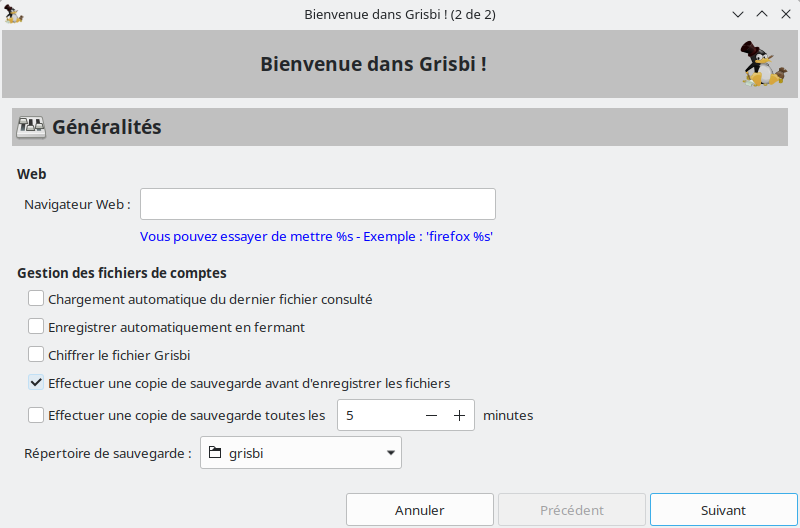
\includegraphics[width=.98\textwidth]{image/screenshot/start_first_launch}
	\end{center}
	\caption{Erstkonfiguration der Kontendatei.}
	\label{start_first_launch}
\end{figure}	
	
Es ist ratsam, die Optionen zu prüfen:%It is advisable to check the options:
	\begin{itemize}
		\item Die letzte Dateï automatisch öffnen;% Automatically load last file on startup%chargement automatique du dernier fichier consulté;
		\item Automatisch speichern;%Automatically save on exit;%enregistrer automatiquement en fermant;
		\item Vor dem Speichern eine Sicherung erstellen (standardmäßig aktiviert).%Make a backup copy before saving files (checked by default).%effectuer une copie de sauvegarde avant d'enregistrer les fichiers (coché par défaut).
	\end{itemize}
\end{enumerate}

\minisec{\textcolor{red}{\strong{Achtung:}}}
Die Grisbi-Entwickler empfehlen, die Option \menu{Datei verschlüsseln} aus den folgenden Gründen nicht zu verwenden:%The Grisbi developers recommend that you do not use the \menu{Encrypt Grisbi file} option for the following reasons:
\begin{itemize}
	\item Es gibt keine Methode zur Wiederherstellung einer verschlüsselten Datei, deren Passwort verloren gegangen ist;%there is no method for recovering an encrypted file whose password has been lost;
	\item Aus einem unbekannten Grund kann die Verwendung dieser Option unter Windows dazu führen, dass die Kontendatei völlig unbrauchbar wird.%For some unknown reason, using this option on Windows can render the accounts file completely unusable.
\end{itemize}  
Es ist jedoch ratsam, regelmäßig Sicherungskopien der unverschlüsselten Datei anzufertigen, wenn Sie sie verwenden.%However, if you use it, it is advisable to make regular back-ups of the unencrypted file.

\begin{enumerate}[resume]
	\item Der zweite Assistent, \dequote{Willkommen zu Grisbi} (oder später \dequote{Assistent für eine neue Datei}), der automatisch auf den ersten folgt, umfasst sechs Schritte, die Ihnen bei der Erstellung der \indexword{Kontodatei}\index{Kontodatei} helfen.%The second wizard, \dequote{Willkommen zu Grisbi} (or later \dequote{New file Assistant}), which automatically follows the first, includes six steps to help you create the \indexword{account file}\index{account file}.%Le deuxième assistant \frquote{Bienvenue dans Grisbi !} (ou plus tard \frquote{Aide à la création d'un nouveau fichier de comptes}), qui suit automatiquement le premier, comprend six étapes qui vous aiderons à la création du \indexword{fichier de comptes}\index{fichier de comptes}.
	\item Darauf folgt automatisch der dritte Assistent, \dequote{Ein neues Konto erstellen}, der zum Erstellen des ersten Kontos verwendet wird und im Abschnitt \ref{start-newfile} unten ausführlich beschrieben wird.%This is followed automatically by the third wizard, \dequote{Create a new account}, which is used to create the first account and is described in detail in section \ref{start-newfile} below.%Puis vient automatiquement le troisième assistant \frquote{Créer un nouveau compte} qui permet de créer le premier compte et qui est décrit en détail dans la section \ref{start-newfile} ci-dessous.
\end{enumerate}

Sie können jeden Assistenten jederzeit mit der Schaltfläche \menu{Abbrechen} verlassen.

Wenn Sie den Erststart-Assistenten nicht verwenden möchten, können Sie stattdessen eine Beispieldatei verwenden (siehe Abschnitt \ref{start-example} unten).

\section{Beispieldatei\label{start-example}}

Wenn Sie Grisbi sofort benutzen wollen, ohne die komplette Einrichtung durchlaufen zu müssen, zum Beispiel um eine Vorstellung von den Möglichkeiten dieses Programms zu bekommen, können Sie die Datei \file{Example\_3.0-de.gsb} von der \lang{Sourceforge.net}\footnote{\urlSourceForgeDocumentation{}} Website im Ordner \dequote{textsf{examples}} herunterladen.

\vspacepdf{5mm}
\textbf{Notiz}: In dieser Beispieldatei sind die Namen der Zahlungsempfänger usw. reine Erfindung; jede Ähnlichkeit mit einer realen Person oder einem realen Unternehmen ist rein zufällig.%{Note}: in this example file, the names of the payees etc are pure invention; any similarity with a real person or business is entirely accidental.

\section{Erstellen einer neuen Kontodatei\label{start-newfile}}

Wenn Sie Grisbi zum ersten Mal verwenden, müssen Sie eine erste \indexword{Kontendatei}\index{Kontendatei} erstellen. Die \gls{Dateinamenserweiterung} lautet \file{.gsb} und der Dateiname \file{Name-ihrer-Datei.gsb}.%The \gls{extension} of this file will be \file{.gsb} and its name will be \file{your-file-name.gsb}.

Unmittelbar danach müssen Sie mindestens ein Konto (Bank-, Geld-, Passiv- oder Aktivkonto, beschrieben im Kapitel Kontoverwaltung) und einige weitere Konten (Giro-, Spar-, Kredit-, eventuell ein \vref{accounts} \menu{Verwaltung von Konten} und einige Übergangskonten) anlegen, die ihre jeweiligen Transaktionen enthalten werden.%Immediately afterwards, you will need to create at least one account (bank, cash, liability or asset account, described in the chapter \vref{accounts} \menu{Account management}), and then a few other accounts (current, savings, credit, possibly a cash account and a few transition accounts) which will contain their respective transactions.

Bei einer Familienverwaltung haben Sie normalerweise nur eine einzige Kontodatei, da dies den gesamten Austausch zwischen Ihren verschiedenen Konten ermöglicht. Wenn Sie einen Verein oder eine weitere Familie verwalten, die in keinem buchhalterischen Zusammenhang mit der ersten Familie steht, erstellen Sie eine weitere Kontodatei, die einen anderen Namen trägt \file{name-ihrer-zweiten-datei.gsb}. Dadurch bleiben die \indexword{Buchhaltungseinheiten}\index{Buchungsberechtigung} getrennt. %If you are managing a family, you will normally only have one accounts file, as this allows all the exchanges between your different accounts. If you are managing an association, or another family with no accounting relationship with the first, you will create another accounts file, which will have a different name your-second-file-name.gsb. This will keep the \indexword{accounting entities}\index{accounting entity} separate.

Mit anderen Worten: Alle Konten Ihres Haushalts werden in einer Kontendatei erfasst, alle Konten Ihrer Vereinigung in einer anderen Kontendatei.


			% TODO update screenshots and text "start", uncomment when finished
%\cleardoubleemptypage

%\include{05-grisbi-manuel-home-de}			% TODO update screenshots and text "home", uncomment when finished
%\cleardoubleemptypage

%\include{06-grisbi-manuel-QIF-de}			% TODO update screenshots and text "QIF", uncomment when finished
%\cleardoubleemptypage

%\include{07-grisbi-manuel-datamanagement-de}	% TODO update screenshots and text "datamanagement", uncomment when finished
%\cleardoubleemptypage

%\include{08-grisbi-manuel-accounts-de}		% TODO update screenshots and text "accounts", uncomment when finished
%\cleardoubleemptypage

%\include{09-grisbi-manuel-transactions-de}	% TODO update screenshots and text "transactions", uncomment when finished
%\cleardoubleemptypage

%\include{10-grisbi-manuel-reconciliation-de}	% TODO update screenshots and text "reconciliation", uncomment when finished
%\cleardoubleemptypage

%\include{11-grisbi-manuel-planned-de}		% TODO update screenshots and text "planned", uncomment when finished
%\cleardoubleemptypage

%\include{12-grisbi-manuel-search-de}			% TODO update screenshots and text "search", uncomment when finished
%\cleardoubleemptypage

%\include{13-grisbi-manuel-third-de}			% TODO update screenshots and text "third", uncomment when finished
%\cleardoubleemptypage

%\include{14-grisbi-manuel-categories-de}		% TODO update screenshots and text "categories", uncomment when finished
%\cleardoubleemptypage

%\include{15-grisbi-manuel-budgetlines-de}	% TODO update screenshots and text "budgetlines", uncomment when finished
%\cleardoubleemptypage

%\include{16-grisbi-manuel-financialyear-de}	% TODO update screenshots and text "financialyear", uncomment when finished
%\cleardoubleemptypage

%\include{17-grisbi-manuel-credit-de}			% TODO update screenshots and text "credit", uncomment when finished
%\cleardoubleemptypage

%\include{18-grisbi-manuel-budget-de}			% TODO update screenshots and text "budget", uncomment when finished
%\cleardoubleemptypage

%\include{19-grisbi-manuel-bankcardmanagement-de}	% TODO update screenshots and text "bankcardmanagement", uncomment when finished
%\cleardoubleemptypage

%\include{20-grisbi-manuel-association}		% fr version only
%\cleardoubleemptypage

%\include{21-grisbi-manuel-reports-de}			% TODO update screenshots and text "reports", uncomment when finished
%\cleardoubleemptypage

%\include{22-grisbi-manuel-reports-creation-de}	% TODO update screenshots and text "reports-creation", uncomment when finished
%\cleardoubleemptypage

%\include{23-grisbi-manuel-setup-de}				% TODO update screenshots and text "setup", uncomment when finished
%\cleardoubleemptypage

%\include{24-grisbi-manuel-maintenance-de}		% TODO update screenshots and text "maintenance", uncomment when finished
%\cleardoubleemptypage



%% Files editors not used anymore, so useless 
%%\include{grisbi-manuel-todo}
%%\cleardoubleemptypage
%
%% Files editors not used anymore, so useless 
%%\include{grisbi-manuel-problems}
%%\cleardoubleemptypage
%
%% Useless so don't include it
%%\include{grisbi-manuel-XML}
%
%% Useless so don't include it
%%\include{grisbi-manuel-FDL}


% Prints the index
\printindex


% Displays a note at the beginning of the glossary
\renewcommand{\glossarypreamble}{\textbf{Notiz}: die meisten Definitionen der Einträge in diesem Glossar stammen aus den gleichnamigen Artikeln der freien und kollaborativen Enzyklopädie \lang{Wikipédia}\footnote{\urlWikipedia{}}. Obwohl diese Texte verändert und an den besonderen Kontext dieses Glossars angepasst wurden, dankt der Autor Wikipedia für die Bereitstellung dieser Referenzen.\newline}


% Prints the glossary
% For pdf only; redefined in hva/macros.hva by an empty command in html
\printglossaries


\end{document}



